% Options for packages loaded elsewhere
\PassOptionsToPackage{unicode,pdfusetitle}{hyperref}
\PassOptionsToPackage{hyphens}{url}
\PassOptionsToPackage{dvipsnames,svgnames*,x11names*}{xcolor}

\documentclass[10pt]{beamer}
\usepackage{lmodern}
\usepackage{amssymb,amsmath,mathtools,amsthm}
\usepackage[T1]{fontenc}
\usepackage[utf8]{inputenc}
\usepackage{textcomp} % provide euro and other symbols

\usepackage{pgfpages}

% prevent slide breaks in the middle of a paragraph
\widowpenalties 1 10000
%\raggedbottom

% redefine part, section, and subsection headers
%\raggedbottom
\setbeamertemplate{part page}{
 \centering
 \begin{beamercolorbox}[sep=16pt,center]{part title}
    \usebeamerfont{part title}\insertpart\par
 \end{beamercolorbox}
}
\setbeamertemplate{section page}{
 \centering
 \begin{beamercolorbox}[sep=12pt,center]{part title}
    \usebeamerfont{section title}\insertsection\par
 \end{beamercolorbox}
}
\setbeamertemplate{subsection page}{
 \centering
 \begin{beamercolorbox}[sep=8pt,center]{part title}
    \usebeamerfont{subsection title}\insertsubsection\par
 \end{beamercolorbox}
}

\AtBeginPart{\frame{\partpage}}
\AtBeginSection{\ifbibliography\else\frame{\sectionpage}\fi}
\AtBeginSubsection{\frame{\subsectionpage}}

% beamer configuration
\usecolortheme{dove}
\usefonttheme{professionalfonts}
\usefonttheme{structurebold}
\setbeamertemplate{footline}[frame number]
\setbeamertemplate{caption}[numbered]
\setbeamertemplate{caption label separator}{: }
\setbeamercolor{caption name}{fg=normal text.fg}
\setbeamertemplate{frametitle}{\begin{centering}\insertframetitle\par\end{centering}}
\setbeamertemplate{itemize items}[circle]
\setbeamerfont{frametitle}{size=\large}
\setbeamertemplate{headline}{\vskip5ex}
\beamertemplatenavigationsymbolsempty
%\setlength{\parskip}{1em} % add paragraph spacing

% Use upquote if available, for straight quotes in verbatim environments
\usepackage{upquote}
\usepackage[]{microtype}
\UseMicrotypeSet[protrusion]{basicmath} % disable protrusion for tt fonts

\usepackage{xcolor}
\usepackage{xurl} % add URL line breaks if available
\usepackage{bookmark}
\usepackage{hyperref}
\hypersetup{
  colorlinks=true,
  linkcolor=Maroon,
  filecolor=Maroon,
  citecolor=Blue,
  urlcolor=Blue
}

\usepackage[inline]{asymptote}

\usepackage{tikz}
\usetikzlibrary{arrows,shapes,positioning,intersections}

\usepackage{pgfplots}
\usepgfplotslibrary{external,colormaps}
\pgfplotsset{width=7cm,compat=1.11}
%\tikzexternalize

%\usepackage{tikz}
%\usepackage{pgfplots}
%\usepackage[mode=buildnew]{standalone}% requires -shell-escape
%\usetikzlibrary{intersections}

\urlstyle{same} % disable monospaced font for URLs
\newif\ifbibliography
\setlength{\emergencystretch}{3em} % prevent overfull lines
\setcounter{secnumdepth}{-\maxdimen} % remove section numbering

%\usepackage{subfig}
\usepackage{subcaption}
\usepackage{algorithm,algpseudocode}
\usepackage{booktabs}
\DeclareMathOperator{\E}{\text{E}}
\DeclareMathOperator{\Var}{var}
\DeclareMathOperator{\Cov}{cov}

% biblatex
\usepackage[citestyle=authoryear]{biblatex}
\addbibresource{ml-group-slope.bib}

\title{SLOPE}
\subtitle{Presentation for the ML group at LUSEM}
\author{Johan Larsson}
\date{May 27, 2020}
\institute{Department of Statistics, Lund University}
\titlegraphic{
\includegraphics{lu.pdf}}

\begin{document}
\frame[noframenumbering,plain]{\titlepage}

\begin{frame}{Overview}
\tableofcontents
\end{frame}

\section{Introducing SLOPE}

\begin{frame}{Motivation and setting}
\protect\hypertarget{sorted-l1}{}
\begin{block}{setting}
    want to apply a \alert{generalized linear model}\footnote{least-squares, logistic, multinomial, or Poisson regression for instance} to a set of predictors \(X \in \mathbb{R}^{n\times p}\) and outcome
    \(y \in \mathbb{R}^n\)\medskip
    
    leads to finding the optimal solution (\(\hat\beta\)) to the problem
    \[
        \text{minimize} \quad g(\beta;X,y),
    \]
    for instance \(g(\beta; X,y) \coloneqq \frac 12 \lVert y - X\beta \rVert_2^2\) for OLS.
\end{block}
\pause
\begin{block}{problem}
\begin{itemize}
    \item \(p \gg n\)
    \item believe \alert{real} \(\beta\) is sparse: few signals, much noise
    \item want to avoid overfitting
    \item want efficiency
\end{itemize}
\end{block}
\end{frame}

\begin{frame}{Regularization}
\begin{block}{idea}
introduce regularization by constraining the problem, i.e. solve
\[
    \begin{aligned}
        &\text{minimize}   && g(\beta;X,y)\\
        &\text{subject to} && h(\beta) \leq t
    \end{aligned}
\]
and choose \(h(\beta)\) such that the resulting model is \alert{sparse} by shrinking some 
elements in \(\beta\) to be \emph{exactly} zero.
\end{block}
\begin{block}{typical choices for \(h(\beta)\)}
\begin{description}
    \item[\(\ell_0\) norm] best subset selection
    \item[\(\ell_1\) norm] the lasso
\end{description}
\end{block}
\end{frame}

\begin{frame}{Problems with standard methods}
\begin{block}{best subset selection}
\begin{itemize}
    \item not convex and therefore intractable for large \(p\)
    \item no shrinkage
\end{itemize}
\end{block}
\begin{block}{lasso}
\begin{itemize}
    \item unpredictable model selection for highly correlated predictors
    \item can only select \(n\) coefficients
\end{itemize}
\end{block}
\end{frame}

\begin{frame}{SLOPE}
\textcite{bogdan2015} introduced SLOPE (Sorted L-One Penalized Estimation), which solves
the problem
\[
\begin{aligned}
    &\text{minimize}   && g(\beta; X,y) \\
    &\text{subject to} && \sum_{i=1}^n \lambda_i \lvert \beta \rvert_{(i)} \leq t,
\end{aligned}
\]
where \(\sum_{i=1}^p\lambda_i \lvert \beta \rvert_{(i)}\) is the \alert{sorted \(\ell_1\) norm},
for which
\[\lambda_1 \geq \lambda_2 \geq \cdots \geq \lambda_p \geq 0\]
and
\[\lvert \beta \rvert_{(1)} \geq \lvert \beta \rvert_{(2)} \geq \cdots \geq \lvert \beta \rvert_{(p)}.\]
\end{frame}

\begin{frame}[fragile]{A step back: least squares}

for simplicity, let's assume \[g(\beta;X,y) = \frac 12 \lVert X\beta - y\rVert_2^2,\] i.e., we 
are solving (unregularized) OLS---solution available analytically through
normal equations.

\begin{center}
\begin{asy}
    import graph;
    import contour;
    
    size(180, 180);
    
    pair x0 = (1.6, 0.8);
    
    dot(x0);
    draw(circle(x0, 0.822), dashed);
    draw(circle(x0, 1.3), dashed);
    draw(circle(x0, 0.344), dashed);
    
    pair p1 = (1.6, 0.8);
    dot("$\hat\beta$", p1);
    
    xaxis("$\beta_1$", xmin = -1.1);
    yaxis("$\beta_2$", ymin = -1.1);
\end{asy}
\end{center}
\end{frame}

\begin{frame}[fragile]{Constraint region for the sorted \(\ell_1\) norm}
\(\sum_{i=1}^p \lambda_i \lvert \beta \rvert_{(i)} \leq t\) defines a 
constraint region centered at \(\boldsymbol{0}\)
\begin{center}
\begin{asy}
    import graph;
    import contour;
    
    size(150, 150);
    
    path p = (-1,0)--(-0.75,0.75)--
             (0,1)--(0.75,0.75)--
             (1,0)--(0.75,-0.75)--
             (0,-1)--(-0.75,-0.75)--(-1,0);
    draw(p);
    
    xaxis("$\beta_1$", xmax = 1.2, xmin = -1.2);
    yaxis("$\beta_2$", ymin = -1.2, ymax = 1.2);
\end{asy}
\end{center}
\end{frame}

\begin{frame}[fragile]{Sorted \(\ell_1\)-regularized least squares}
    let's introduce regularization via the sorted \(\ell_1\) norm: solution \(\hat\beta\)
    has to lie inside constraint region defined by 
    \[\sum_{i=1}^p \lambda_i\lvert \beta \rvert_{(i)} \leq t.\]
    \begin{center}
        \begin{asy}
            import graph;
            import contour;
            
            size(180, 180);
            
            path p = (-1,0)--(-0.75,0.75)--
                     (0,1)--(0.75,0.75)--
                     (1,0)--(0.75,-0.75)--
                     (0,-1)--(-0.75,-0.75)--(-1,0);
            draw(p);
            draw(scale(0.5)*p);
            
            pair x0 = (1.6, 0.8);
            
            dot(x0);
            draw(circle(x0, 0.822), dashed);
            draw(circle(x0, 1.3), dashed);
            draw(circle(x0, 0.344), dashed);
            
            pair p1 = (0.75/2, 0.75/2);
            dot("$\beta^*_{\lambda^{(1)}}$", p1);
            
            pair p2 = (0.805, 0.59);
            dot("$\beta^*_{\lambda^{(2)}}$", p2);
            
            xaxis("$\beta_1$", xmin = -1.1);
            yaxis("$\beta_2$", ymin = -1.1);
        \end{asy}
    \end{center}
\end{frame}

\begin{frame}[fragile]{Shapes of the sorted \(\ell_1\) norm}
    choice of \(\lambda\) dictates shape of the constraint region
    \begin{figure}[hbtp]
        \begin{subfigure}[b]{.3\linewidth}
            \centering
            \begin{asy}
                import graph;
                import contour;
                
                size(80, 80);
                
                path p = (-1,0)--(0,1)--(1,0)--(0,-1)--(-1,0);
                draw(p);
                xaxis("$\beta_1$", xmax = 1.5, xmin = -1.1);
                yaxis("$\beta_2$", ymax = 1.5, ymin = -1.1);
            \end{asy}
            \caption{\(\lambda_1 = \lambda_2\)}
        \end{subfigure}
        \begin{subfigure}[b]{.3\linewidth}
            \begin{asy}
                import graph;
                import contour;
                
                size(80, 80);
                
                path p = (-1,0)--(-0.75,0.75)--
                         (0,1)--(0.75,0.75)--
                         (1,0)--(0.75,-0.75)--
                         (0,-1)--(-0.75,-0.75)--(-1,0);
                draw(p);
                xaxis("$\beta_1$", xmin = -1.1, xmax = 1.5);
                yaxis("$\beta_2$", ymin = -1.1, ymax = 1.5);
            \end{asy}
            \caption{\(\lambda_1 > \lambda_2 > 0\)}
        \end{subfigure}
        \begin{subfigure}[b]{.3\linewidth}
            \begin{asy}
                import graph;
                import contour;
                
                size(80, 80);
                
                path p = (-1,0)--(-1,1)--(1,1)--(1,-1)--(-1,-1)--(-1,0);
                draw(p);
                xaxis("$\beta_1$", xmin = -1.1, xmax = 1.5);
                yaxis("$\beta_2$", ymin = -1.1, ymax = 1.5);
            \end{asy}
        \caption{\(\lambda_1 > \lambda_2 = 0\)}
    \end{subfigure}
    %\caption{Shapes of the sorted \(\ell_1\) norm}
    \end{figure}
\end{frame}

\begin{frame}{Equivalent formulations}

We've so far defined SLOPE as the \alert{constrained} optimization problem
\[
\begin{aligned}
    &\text{minimize}   && g(\beta; X) \\
    &\text{subject to} && \sum_{i=1}^p \lambda_i \lvert \beta \rvert_{(i)} \leq t,
\end{aligned}
\]
but, with a bit of notational abuse\footnote{Redefining \(\lambda\).}, this is equivalent to the \alert{unconstrained} problem
\[
\text{minimize} \quad g(\beta;\lambda) + J(\beta;\lambda),
\]
with \(J(\beta;\lambda) = \sum_{i=1}^p \lambda_i|\beta|_{(i)}\).
\end{frame}

\begin{frame}{Clustering Property}
    The sorted \(\ell_1\) norm induces clustering: setting absolute values of coefficients
    to same value\medskip
    
    Consider the two-dimensional case \(y = x_1\beta_1 + x_2\beta_2 + \varepsilon\).
    \begin{table}[htb]
        \centering
        
        \begin{tabular}{cc}
            \toprule
             lasso & SLOPE \\
             \midrule
             \(\lambda|\beta_1| + \lambda|\beta_2|\) & \(\lambda_1 |\beta|_{(1)} + \lambda_2 |\beta|_{(2)}\)\\
             \bottomrule
        \end{tabular}
    \end{table}
    and assume \(x_1\) and \(x_2\) are perfectly correlated, then
    \begin{itemize}
        \item the lasso will force one of the coefficients to zero, whilst
        \item SLOPE (provided \(\lambda_1 > \lambda_2 \geq 0\)) will set them to the same value.
    \end{itemize}
\end{frame}

\section{Selection of Regularization Sequence}

\begin{frame}[fragile]{Choice of \(\lambda\)}
\begin{itemize}
    \item \(\lambda\) is \(p\)-dimensional, which means there is \alert{considerable} 
          freedom in choosing it
    \item to make this problem manageable, we therefore assume that each \(\lambda_i\)
          is a function of \(p\), \(n\), \(i\), and some parameters
\end{itemize}
\end{frame}

\begin{frame}{Choice of \(\lambda\): BH}

\begin{columns}[T]
\begin{column}{0.45\linewidth}
    Inspiration for SLOPE comes from the desire to
    control of false discovery rate (FDR) in a regression setting, i.e.
    test the hypotheses
    \[
        H_{0,j}: \beta_j = 0 \qquad H_{1,j}: \beta_j \neq 0.
    \]
    
    \begin{block}{Benjamini--Hochberg (BH) procedure}
        Sort \(\hat\beta\) in non-decreasing order according to its absolute values and reject all hypothesis \(H_{(i)}\) for which \(i \leq i_{\text{BH}}\), where
        \[
            i_\text{BH} = \max\left\{i \mid |\hat\beta|_{(i)} \geq \sigma\Phi^{-1}\left(1 - \frac{iq}{2p}\right)\right\},
        \]
        where \(\Phi^{-1}\) is the probit function.
    \end{block}
\end{column}
\begin{column}{0.45\linewidth}
    \begin{figure}
        \centering
        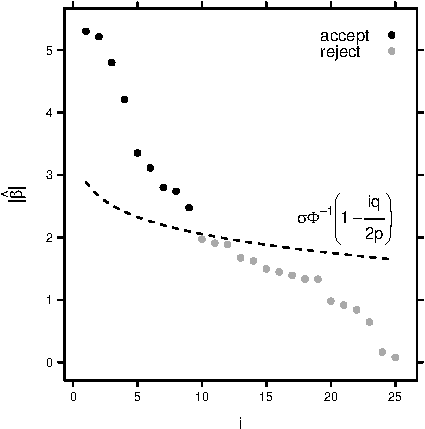
\includegraphics[width=\linewidth]{figures/bh.pdf}
        \caption{BH correction.}
    \end{figure}
\end{column}
\end{columns}
\end{frame}

\begin{frame}{BH \(\lambda\) method for SLOPE}

The BH method for choosing the \(\lambda\) sequence in SLOPE sets
\[\lambda_i = \sigma\Phi^{-1}\left(1 - \frac{qi}{2p}\right).\]
Very similar to procedure from last slide.\medskip

It turns out that this sequence promises FDR control in \alert{orthogonal} settings \autocite[Theorem 1.1]{bogdan2015}, namely
\[
    \text{FDR}  \leq \frac{qp_0}{p},
\]
where \(p_0\) is the number of true null hypotheses. In other words, \(q\) sets an upper bound on FDR.
\end{frame}

\begin{frame}{FDR, Power, and Prediction Error}

Results from debiased\footnote{Select support using SLOPE or lasso and estimate coefficients using standard OLS.} SLOPE and lasso and cross-validated lasso show that SLOPE controls FDR as promised and has better predictive performance.

\begin{figure}
    \centering
    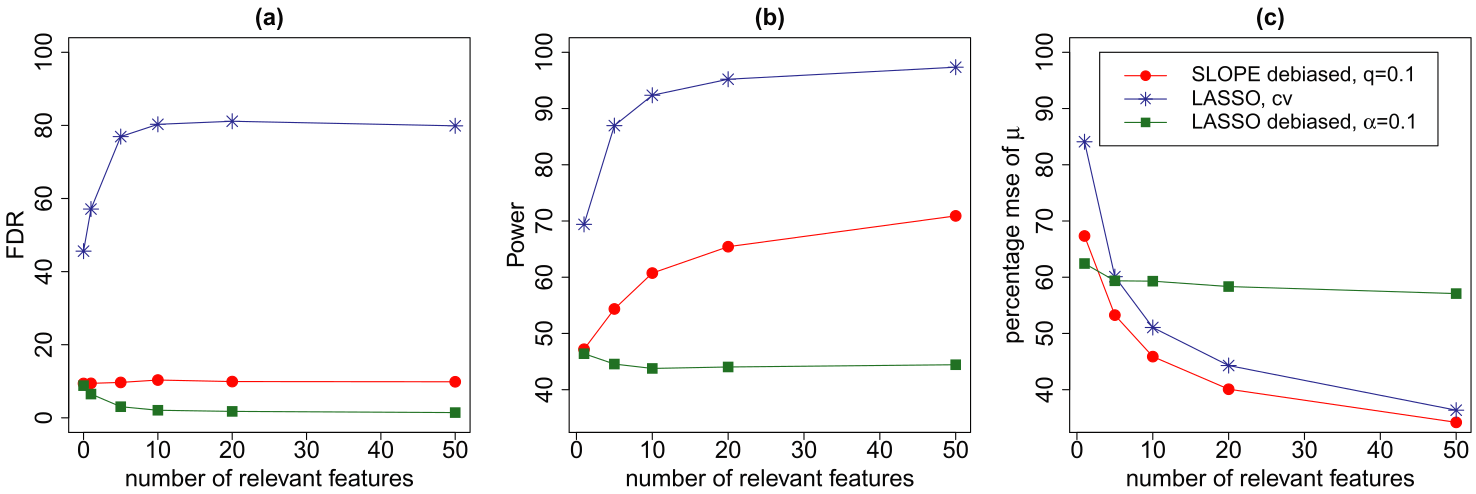
\includegraphics[width=\linewidth]{figures/bogdan-fig2.png}
    \caption{FDR, power, and mean-squared error (MSE) for lasso SLOPE using BH sequence. Predictors are i.i.d. generated from a normal distribution.}
\end{figure}
\end{frame}

\begin{frame}{FDR in Gaussian design}

When design is \alert{not} orthogonal, SLOPE with the BH sequence loses control of FDR
as the number of relevant predictors increase.

\begin{figure}
    \centering
    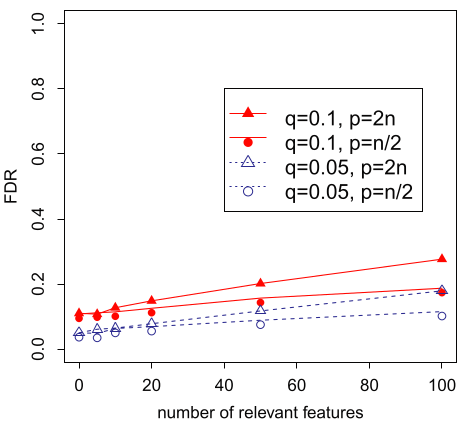
\includegraphics[width=0.5\linewidth]{figures/bogdan-fig5.png}
    \caption{FDR control for SLOPE with BH sequence for Gaussian i.i.d. design. \(p = 2n = 10000\).}
\end{figure}
\end{frame}

\begin{frame}{Choice of \(\lambda\): Gaussian Sequence}

In light of the problem with FDR control for non-orthogonal settings, \textcite{bogdan2015} consider also the \alert{Gaussian} sequence that sets
\[\lambda_i = \min\left(\lambda_{i-1}, \lambda^{\mathrm{BH}}_i\sqrt{1 + \frac{1}{n-i} \sum_{j < i}\lambda_i^2}\right),\]

\begin{columns}[T]
\begin{column}{0.35\linewidth}
which flattens out the sequence based on $n/p$ fraction.\medskip

Note, however, that for \(p \gg n\), this sequence reduces to the lasso.
\end{column}
\begin{column}{0.55\linewidth}
    \begin{figure}
    \centering
    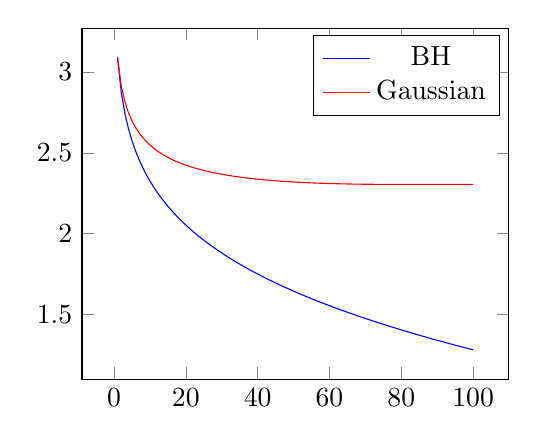
\begin{tikzpicture}
\begin{axis}[no marks]
    \addplot+
        coordinates {
            (1,3.090232306167818)
            (2,2.878161739095489)
            (3,2.747781385444999)
            (4,2.652069807902201)
            (5,2.5758293035489053)
            (6,2.5121443279304674)
            (7,2.457263390205441)
            (8,2.4089155458154656)
            (9,2.3656181268642973)
            (10,2.326347874040846)
            (11,2.2903678778552723)
            (12,2.25712924448623)
            (13,2.22621176931718)
            (14,2.1972863766410575)
            (15,2.170090377584565)
            (16,2.1444106209118456)
            (17,2.120071689742156)
            (18,2.0969274291643467)
            (19,2.074854734393314)
            (20,2.0537489106318274)
            (21,2.033520149253055)
            (22,2.0140908120181424)
            (23,1.9953933101678294)
            (24,1.9773684281819504)
            (25,1.9599639845400576)
            (26,1.9431337511050712)
            (27,1.9268365732639148)
            (28,1.9110356475491233)
            (29,1.8956979239918437)
            (30,1.8807936081512553)
            (31,1.8662957434581111)
            (32,1.8521798587690468)
            (33,1.8384236692477764)
            (34,1.8250068211464028)
            (35,1.8119106729525973)
            (36,1.799118106837967)
            (37,1.78661336549347)
            (38,1.7743819103449572)
            (39,1.7624102978623892)
            (40,1.7506860712521692)
            (41,1.7391976652852517)
            (42,1.7279343223884185)
            (43,1.7168860184310402)
            (44,1.706043396888962)
            (45,1.695397710272136)
            (46,1.6849407678719142)
            (47,1.6746648890243248)
            (48,1.6645628612027212)
            (49,1.6546279023510773)
            (50,1.6448536269514717)
            (51,1.6352340153886495)
            (52,1.6257633862332344)
            (53,1.6164363711150214)
            (54,1.6072478919002173)
            (55,1.598193139922817)
            (56,1.5892675570513919)
            (57,1.580466818399361)
            (58,1.5717868165098592)
            (59,1.5632236468662757)
            (60,1.5547735945968535)
            (61,1.5464331222567473)
            (62,1.538198858584064)
            (63,1.530067588137829)
            (64,1.5220362417358557)
            (65,1.5141018876192844)
            (66,1.5062617232782438)
            (67,1.4985130678799756)
            (68,1.4908533552466605)
            (69,1.4832801273356209)
            (70,1.4757910281791704)
            (71,1.4683837982456598)
            (72,1.4610562691869062)
            (73,1.453806358940575)
            (74,1.4466320671589783)
            (75,1.4395314709384566)
            (76,1.432502720825811)
            (77,1.425544037080452)
            (78,1.4186537061727382)
            (79,1.4118300775008086)
            (80,1.4050715603096327)
            (81,1.3983766207974957)
            (82,1.3917437793963248)
            (83,1.3851716082134353)
            (84,1.3786587286232777)
            (85,1.372203808998726)
            (86,1.3658055625722716)
            (87,1.3594627454182584)
            (88,1.353174154548003)
            (89,1.3469386261102796)
            (90,1.3407550336902165)
            (91,1.3346222867001933)
            (92,1.3285393288568097)
            (93,1.3225051367384355)
            (94,1.3165187184182603)
            (95,1.310579112168129)
            (96,1.3046853852287899)
            (97,1.2988366326425056)
            (98,1.2930319761442424)
            (99,1.2872705631079422)
            (100,1.2815515655446004)
        }
        ;
    \addlegendentry {BH}
    \addplot+
        coordinates {
            (1,3.090232306167818)
            (2,2.9173845779035155)
            (3,2.818382685246308)
            (4,2.7499239113201455)
            (5,2.6982261870995816)
            (6,2.6571074135940767)
            (7,2.623259133663289)
            (8,2.5947043244243506)
            (9,2.5701681349080747)
            (10,2.5487811919309307)
            (11,2.5299246106958906)
            (12,2.5131425538521555)
            (13,2.4980898432276213)
            (14,2.484499017344542)
            (15,2.4721587755049)
            (16,2.4608993940461668)
            (17,2.4505825754377093)
            (18,2.4410942077784727)
            (19,2.432339088970471)
            (20,2.4242370097411317)
            (21,2.416719796826025)
            (22,2.4097290476181126)
            (23,2.4032143713198613)
            (24,2.397132006831161)
            (25,2.3914437247585605)
            (26,2.3861159464129926)
            (27,2.381119030441479)
            (28,2.376426690336332)
            (29,2.372015515120872)
            (30,2.367864572105775)
            (31,2.363955075471549)
            (32,2.3602701080565938)
            (33,2.3567943864599736)
            (34,2.353514061643854)
            (35,2.350416548813963)
            (36,2.3474903815892154)
            (37,2.3447250864336535)
            (38,2.342111074079678)
            (39,2.339639545269844)
            (40,2.3373024086210488)
            (41,2.335092208797028)
            (42,2.3330020634830957)
            (43,2.331025607906938)
            (44,2.3291569458528563)
            (45,2.327390606283717)
            (46,2.3257215048222486)
            (47,2.3241449094568516)
            (48,2.3226564099314984)
            (49,2.321251890357946)
            (50,2.319927504654405)
            (51,2.318679654470179)
            (52,2.317504969302526)
            (53,2.316400288551544)
            (54,2.3153626452924887)
            (55,2.314389251573557)
            (56,2.3134774850716338)
            (57,2.3126248769595166)
            (58,2.311829100856128)
            (59,2.3110879627467935)
            (60,2.3103993917741263)
            (61,2.309761431811675)
            (62,2.309172233742638)
            (63,2.3086300483747513)
            (64,2.3081332199301476)
            (65,2.307680180055741)
            (66,2.3072694423055164)
            (67,2.306899597051429)
            (68,2.3065693067839805)
            (69,2.3062773017677887)
            (70,2.3060223760208163)
            (71,2.3058033835892373)
            (72,2.3056192350925926)
            (73,2.305468894516453)
            (74,2.30535137623195)
            (75,2.305265742223562)
            (76,2.305211099508238)
            (77,2.3051865977305903)
            (78,2.3051865977305903)
            (79,2.3051865977305903)
            (80,2.3051865977305903)
            (81,2.3051865977305903)
            (82,2.3051865977305903)
            (83,2.3051865977305903)
            (84,2.3051865977305903)
            (85,2.3051865977305903)
            (86,2.3051865977305903)
            (87,2.3051865977305903)
            (88,2.3051865977305903)
            (89,2.3051865977305903)
            (90,2.3051865977305903)
            (91,2.3051865977305903)
            (92,2.3051865977305903)
            (93,2.3051865977305903)
            (94,2.3051865977305903)
            (95,2.3051865977305903)
            (96,2.3051865977305903)
            (97,2.3051865977305903)
            (98,2.3051865977305903)
            (99,2.3051865977305903)
            (100,2.3051865977305903)
        }
        ;
    \addlegendentry {Gaussian}
\end{axis}
\end{tikzpicture}

\end{figure}
\end{column}
\end{columns}

\end{frame}

\begin{frame}{FDR Control with Gaussian Sequence}
    Gaussian sequence does a better job of controlling FDR in the Gaussian (but i.i.d.) case.
    
    \begin{figure}
        \centering
        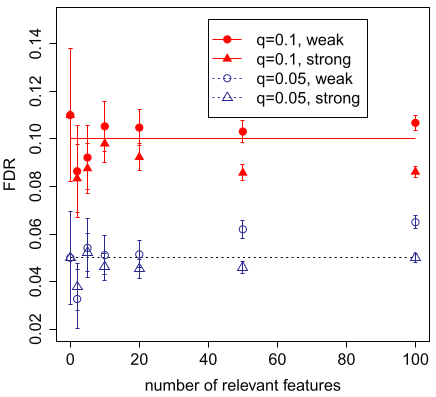
\includegraphics[width=0.5\linewidth]{figures/bogdan-fig7.png}
        \caption{FDR control for SLOPE with Gaussian sequence for Gaussian i.i.d. design. \(p = 2n = 10000\).}
    \end{figure}
\end{frame}

\section{Parameter Selection for Regularization Sequence}

\begin{frame}[fragile]{Selecting parameters for \(\lambda\) sequence}
We've reduced the problem of specifying the entire \(\lambda\) sequence to specifying parameters \(\sigma\) and \(q\) but \alert{how do we choose these?}\medskip

\begin{block}{three options}
\begin{enumerate}
    \item we know \(\sigma\) and can assume that predictors are not very correlated
    \item use \autocite[Algorithm 5]{bogdan2015} and estimate \(\sigma\) using SLOPE to select support and OLS estimates to approximate \(\sigma\)
    \item cross-validation
\end{enumerate}
Choice depends on situation. \textbf{1} is of course usually intractable, \textbf{2} works well with low correlation and \(n > p\), \textbf{3} is attractive for prediction properties (but we lose FDR control).
\end{block}
\end{frame}

\begin{frame}{Cross-validation and the regularization path}
    \begin{columns}[c]
        \begin{column}{0.45\linewidth}
        If we are interested in cross-validation to select \(\sigma\) and \(q\), we will generally want to construct a \alert{regularization path} of \(\lambda\) sequences, \[\lambda^{(1)}, \lambda^{(2)}, \dots, \lambda^{(m)}.\]
        
        In addition, we want \(\lambda^{(1)}\) and \(\lambda^{(m)}\) to yield the \alert{intercept-only} model and \alert{almost-saturated} model respectively.\medskip
        
        \begin{block}{tuning parameters}
        \(\sigma\) (scale), \(q\) (shape)
        \end{block}
        \end{column}
        \begin{column}{0.45\linewidth}
            \begin{figure}
                \centering
                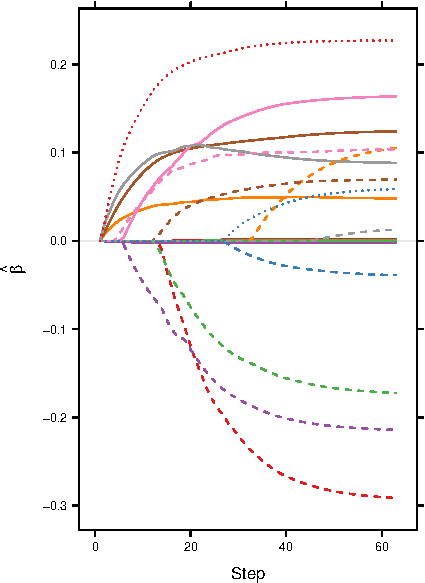
\includegraphics[width=\linewidth]{figures/slope-path.pdf}
                %\caption{Caption}
            \end{figure}
        \end{column}
    \end{columns}
\end{frame}

\section{SLOPE and lasso comparisons}

\begin{frame}{SLOPE and lasso regularization paths}
    \begin{figure}
        \centering
        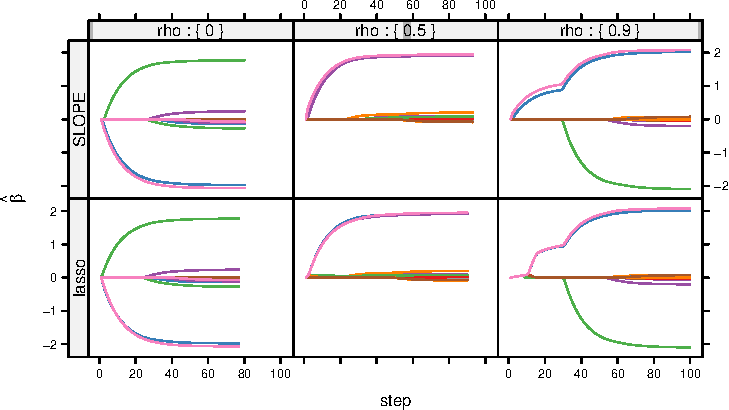
\includegraphics[width=\linewidth]{figures/lassoslopepath.pdf}
        \caption{Comparison of SLOPE and lasso paths for correlated and uncorrelated data.}
    \end{figure}
\end{frame}

\begin{frame}{Grouping effects}
\begin{columns}
\begin{column}{0.45\linewidth}
    Differences between lasso and SLOPE are clear in block-correlated covariance matrices.
    
    \vspace{5ex}
    
    \begin{figure}
        \centering
        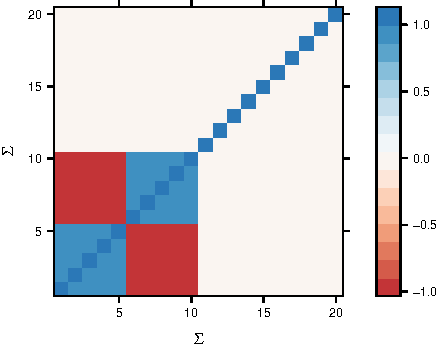
\includegraphics[width=0.8\linewidth]{figures/grouping-effect-sigma.pdf}
        \caption{Correlation structure.}
    \end{figure}
\end{column}
\begin{column}{0.45\linewidth}
    \begin{figure}
        \centering
        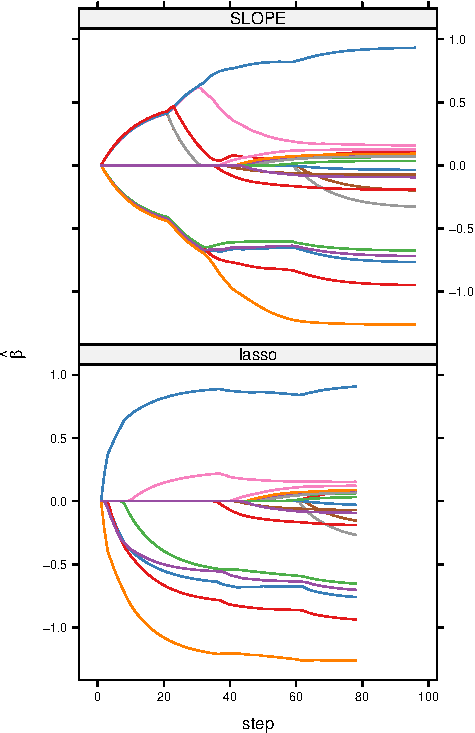
\includegraphics[width=0.9\linewidth]{figures/grouping-effect.pdf}
        \caption{Regularization paths.}
    \end{figure}
\end{column}
\end{columns}
\end{frame}

\begin{frame}{Performance and screening rules}

Sparsity-enforcing methods, such as lasso and SLOPE, can be \alert{very efficient}, particularly when \(p \gg n\) due to \alert{screening rules}\medskip

Screening rules are based on the idea that many solutions along the path will be sparse and that we can estimate this and \alert{discard} predictors before fitting the model.\medskip

We have developed a screening rule for SLOPE~\autocite{larsson2020b}

\end{frame}

\section{SLOPE extensions, implementation, and discussion}

\begin{frame}{Extensions of SLOPE}

Several extensions of SLOPE exists, all analagous to popular
lasso derivatives.

\begin{block}{Adaptive Bayesian SLOPE (ABSLOPE)}
    Semi-Bayesian approach that adapatively reweights penalties. See \textcite{jiang2019}.
\end{block}

\begin{block}{Group SLOPE}
    Sorted \(\ell_1\) norm regularization on group level
    \(\ell_2\) norm regularization on individual level. See \textcite{brzyski2018}.
\end{block}
\end{frame}

\begin{frame}{Software}

Most software is still under development, not quite mature.\medskip

\begin{block}{implementations}
\begin{itemize}
    \item SLOPE: \url{https://CRAN.R-project.org/package=SLOPE}
    \item Group SLOPE: \url{https://CRAN.R-project.org/package=grpSLOPE}
    \item ABSLOPE: \url{https://github.com/wjiang94/ABSLOPE}
\end{itemize}
\end{block}

\end{frame}

\begin{frame}{Topics for discussion}

\begin{itemize}
    \item How interested are you in 
    \begin{itemize}
        \item FDR control?
        \item model selection properties?
        \item prediction properties?
    \end{itemize}
    \item SLOPE penalizes stronger signals more than weaker ones---is this reasonable?
    \item choice of \(\lambda\) sequence has not been thoroughly investigated---any ideas? 
\end{itemize}
    
\end{frame}

\begin{frame}[allowframebreaks]{References}
  \bibliographytrue
  \printbibliography[heading=none]
\end{frame}

\end{document}
